 \documentclass{beamer}
\usepackage[latin1]{inputenc}
\usepackage{amsmath}
\usetheme{Warsaw}

\newcommand\applyFontA{\fontsize{6}{6}\selectfont}
\newcommand\applyFontB{\fontsize{8}{8}\selectfont}

\title[Interest Rate Options]{Caps, Floors and Swaptions}
\author{Michal Mackanic}
\institute{RMO/CZ}
\date{August 2016}

\begin{document}

\begin{frame}
	\titlepage
\end{frame}

\begin{frame}
	\frametitle{Outline}
	\tableofcontents[hideallsubsections]
\end{frame}

\AtBeginSection[]
{
  \begin{frame}<beamer>
    \frametitle{Section}
    \begin{beamercolorbox}[sep=4pt,center]{part title}
		\large{\insertsectionhead}\par%
    \end{beamercolorbox}
  \end{frame}
}

\AtBeginSubsection[]
{
  \begin{frame}<beamer>
    \frametitle{Section}
    \begin{beamercolorbox}[sep=4pt,center]{part title}
		\insertsubsectionhead\par%
    \end{beamercolorbox}
  \end{frame}
}

\AtBeginSubsubsection[]
{
  \begin{frame}<beamer>
    \frametitle{Section}
    \begin{beamercolorbox}[sep=2pt,center]{part title}
		\insertsubsubsectionhead\par%
    \end{beamercolorbox}
  \end{frame}
}

\applyFontB

\section{Symbols Used}

\begin{frame}{Symbols Used}
\begin{tabular}{l l}
IRS & interest rate swap\\
$L$ & underlying notional\\
$\Delta t$ & interest rate period\\
$r$ & current EURIBOR / swap rate quotation\\
$K$ & strike\\
$T$ & time $T$ in years\\
$F_{T - \Delta t, T}$ & forward rate for period $T - \Delta t$ to $T$\\
$F$ & forward rate; period is given by the context\\
$DF_{0,T}$ & discount factor for period $0$ to $T$\\
$\sigma$ & interest rate volatility\\
$N(x)$ & standardized normal cumulative distribution\\
$N'(x)$ & standardized normal probability distribution\\
$r_F$ & risk-free rate\\

\end{tabular}
\end{frame}

\section{Overview of Basic Interest Rate Options}

\begin{frame}{Cap}
\setbeamertemplate{itemize items}[ball]
Cap is an interest rate derivative which protects its owner against interest rate increase.
\setbeamertemplate{itemize items}[ball]
\begin{itemize}
	\item Consider a corporation which takes 5Y loan of 1 MEUR that resets annually to 12M EURIBOR + 120 bps. If it does not want interest rate on the loan to exceed 5.00\%, it will buy a cap with a strike of 3.80\%\footnote{\tiny{Cap is linked to 12M EURIBOR rather than to 12M EURIBOR + 120 bps. Therefore cap strike is to be calculated as 5.00\% - 120bps = 3.80\%}}. Every time 12M LIBOR exceeds 3.80\% on reset date, the cap pays
difference between EURIBOR and strike of 3.80\%.
\end{itemize}

\mbox{}\\
Cap is a series of options, so called caplets, rather than one single option. Number of caplets corresponds to number of reset periods. Each caplet can be modelled as a call option.

\mbox{}\\
Underlying loan is reset at the beginning of each interest period but the interest payment is realised at its end. The same is true for caplets - their pay-off is known at reset time but it is realised only at the end of interest rate period.
\end{frame}

\begin{frame}{Cap}
\begin{figure}[htp]
\centering
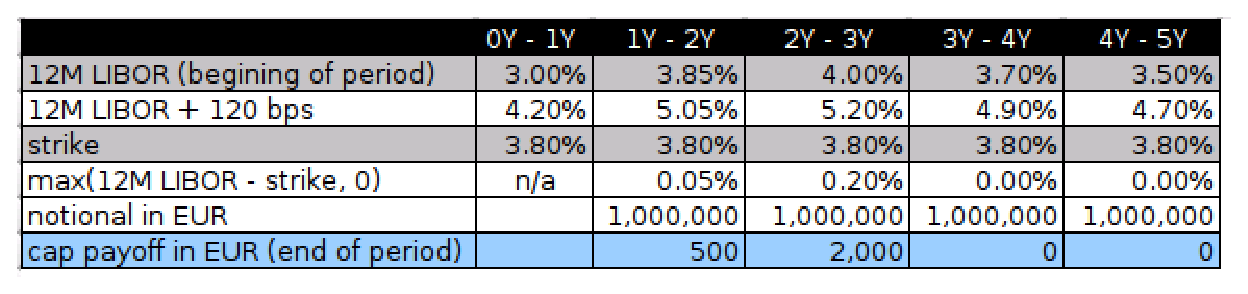
\includegraphics[scale = 0.50]{cap.eps}
\caption{Cap}
\label{cap}
\end{figure}
\end{frame}

\begin{frame}{Floor}
\setbeamertemplate{itemize items}[ball]
Wheares cap protects its owner against intrest rate increase, floor protects its owner against interest rate decrease.
\begin{itemize}
	\item Consider a bank which provides 5Y loan of 1 MEUR reset annually to 12M EURIBOR + 120 bps. If it does not want interest rate on the loan to drop below 2\%, it will buy a floor with a strike of 0.80\%\footnote{\tiny{Similarly to cap, floor strike is calculated as 2.00\% - 120 bps = 0.80\%.}}. Every time 12M EURIBOR drops below 0.80\% on reset date, the floor pays difference between 0.80\% and EURIBOR.
\end{itemize}

\mbox{}\\
Similar to cap, floor is a series of options called floorlets. Floorlets can be modelled as put options.
\end{frame}

\begin{frame}{Floor}
\begin{figure}[htp]
\centering
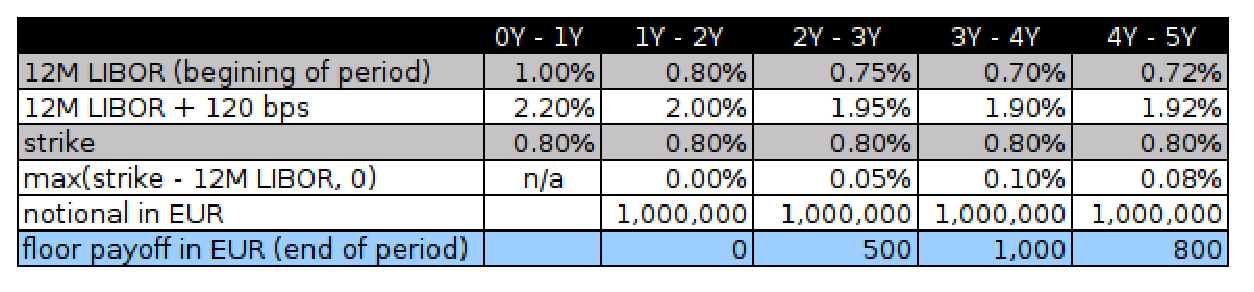
\includegraphics[scale = 0.50]{floor.eps}
\caption{Floor}
\label{floor}
\end{figure}
\end{frame}

\begin{frame}{Cap-Floor Parity}
\setbeamertemplate{itemize items}[ball]
Consider a corporation which takes 5Y loan of a 1 MEUR reset annually to 12M EURIBOR. Let us assume that it buys a cap at strike of 5.00\% and simultaneously sells floor at strike of 5.00\%. The combined pay-off of the two derivatives on a given reset date $t$ will be
\begin{multline}
\textit{pay-off}_t^{~tot} = \textit{pay-off}_t^{~cap} - \textit{pay-off}_t^{~flr} =\\
max(EURIBOR_t^{12M} - 5\%, 0\%) - max(5\% - EURIBOR_t^{12M}, 0\%) =\\
EURIBOR_t^{12M} - 5\% 
\end{multline}
If we further add the loan, which is reset at 12M EURIBOR, we get
\begin{equation}
\textit{pay-off}_t^{~tot*} = EURIBOR_t^{12M} - 5\% - EURIBOR_t^{12M} = -5\%
\end{equation}
Therefore the corporation has effectively converted its floating loan into a fixed one. This could have been achieved through IRS that exchanges 12M EURIBOR for a fixed rate of 5.00\%.
The conclusion of the above is therefore a cap-floor parity in form of
\begin{equation}
cap_t - floor_t = IRS_t
\end{equation}
\end{frame}

\begin{frame}{Swaption}
\setbeamertemplate{itemize items}[ball]
Swaption gives its owner an option to enter a predetermined IRS at some future point in time.
\begin{itemize}
	\item Consider a swaption which enables us to enter 5Y IRS where we (a) receive 6M EURIBOR semiannually and (b) pay fixed interest payment of 3.00\% annually. Let us assume we can exercise the swaption (and therefore enter the underlying IRS) 3Y from now.
	\item If, after 3 years have passed, 5Y swap rate is above 3.00\% we will exercise the swaption since NPV of the underlying IRS will be positive\footnote{\tiny{This certainly must be the case because if we entered a new IRS with NPV = 0, we would have to pay a fixed rate of more than 3.00\% wheares if we exercised the swaption, we would enter underlying IRS where we would pay a fixed rate of only 3.00\%.}}. On contrary, if the swap rate is below 3.00\% we will not exercise the swaption as NPV of the underlying IRS is negative.
\end{itemize}
\end{frame}

\begin{frame}{Swaption}
\setbeamertemplate{itemize items}[ball]
There are two types of swaptions.
\begin{itemize}
	\item In case of receiver swaption its owner pays float and receives fixed interest rate if she decides to enter the underlying IRS. Such an option can be modelled as a call option.
	\item In case of payer swaption its owner pays fixed and receives floating interest rate if she decides to enter the underlying IRS (this is the option we considered above as an example). Such an option can be modelled as a put option.
\end{itemize}
\end{frame}

\section{Black-Scholes Model}

\begin{frame}{Cap}
\setbeamertemplate{itemize items}[ball]
\begin{itemize}
\item Consider a caplet with residual maturity of $T$, underlying notional $L$, strike of $K$ and interest rate period of $\Delta t$. Its pay-off at maturity date $t = T$ is therefore defined as
\begin{equation}
caplet_T = L \cdot \Delta t \cdot max(r - K, 0)
\end{equation}
where $r$ is xIBOR rate that was fixed at the beginning of interest rate period, ie. at $t = T - \Delta t$.
\item Caplet can be treated as a call option. If all Black-Scholes model assumptions hold, its value at $t = 0$ can be calculated as
\begin{equation}
caplet_t = DF_{0, T} \cdot L \cdot \Delta t \cdot \left(F_{T - \Delta T, T} N(d_1) - KN(d_2) \right)
\end{equation}
where $d_1 = \frac{\ln(F_{T - \Delta T, T} - K)}{\sigma \sqrt{T}}$, $d_2 = d_1 - \sigma \sqrt{T}$ and $F_{T - \Delta T, T}$ is a forward rate for period $T - \Delta t$ to $T$ and plays a role of the "best" xIBOR estimate.
\item Since cap is a series of caplets, its value is defined simply as a sum of individual caplets.
\begin{equation}
cap_t = \sum_{i = 1}^n caplet_i = L \cdot \Delta t \sum_{i = 1}^n DF_{0, T_i} \cdot \left(F_{T_i - \Delta t,T_i} N(d_{1i}) - KN(d_{2i}) \right)
\end{equation}
\end{itemize}
\end{frame}

\begin{frame}{Floor}
\setbeamertemplate{itemize items}[ball]
\begin{itemize}
\item Consider a floorlet with residual maturity of $T$, underlying notional $L$, strike of $K$ and interest rate period of $\Delta t$. Its pay-off at maturity date $t = T$ is therefore defined as
\begin{equation}
floorlet_T = L \cdot \Delta t \cdot max(K - r, 0)
\end{equation}
where $r$ is xIBOR rate that was fixed at the beginning of interest rate period, ie. at $t = T - \Delta t$.
\item Floorlet can be treated as a put option. If all Black-Scholes model assumption hold, its value at $t = 0$ can be calculated as
\begin{equation}
floorlet_t = DF_{0, T} \cdot L \cdot \Delta t \cdot \left(KN(-d_2) - F_{T - \Delta T, T} N(-d_1) \right)
\end{equation}
where $d_1 = \frac{\ln(F_{T - \Delta T, T} - K)}{\sigma \sqrt{T}}$, $d_2 = d_1 - \sigma \sqrt{T}$ and $F_{T - \Delta T, T}$ is a forward rate for period $T - \Delta t$ to $T$ and plays a role of the "best" xIBOR estimate.
\item Since floor is a series of floorlets, its value is defined simply as a sum of individual floorlets.
\begin{equation}
floor_t = \sum_{i = 1}^n floorlet_i = L \cdot \Delta t \sum_{i = 1}^n DF_{0, T_i} \cdot \left(KN(-d_{2i}) - F_{T_i - \Delta t, T_i} N(-d_{1i}) \right)
\end{equation}
\end{itemize}
\end{frame}

\begin{frame}{Receiver Swaption}
\setbeamertemplate{itemize items}[ball]
\begin{itemize}
\item Consider a receiver swaption at its maturity date $T$. It is exercised only if $NPV^*$, the value of the underlying IRS, exceeds $NPV$, value of the corresponding IRS concluded at prevailing market conditions, ie. if actual swap rate $r$ exceeds contractual swap rate $K$. Receiver swaption pay-off can be therefore defined as
\begin{equation}
swptn^{rec}_T = max(NPV^* - NPV, 0)
\end{equation}
which can be expanded into
\begin{equation}
swptn^{rec}_T = (L \cdot \Delta t \sum_{i = 1}^n DF_{0, T_i})max(r - K, 0)
\end{equation}
where $L$ stands for IRS notional, $\Delta t$ is interest rate period of the IRS fixed leg, $n$ is number of interest rate periods and $DF_{0, T_i}$ represents discount factor.
\item If all assumptions of Black-Scholes model are fulfilled, a swaption value at $t = 0$ can be calculated as
\begin{equation}
swptn^{rec} = (L \cdot \Delta t \sum_{i = 1}^n DF_{0, T_i}) \left(FN(d_1) - KN(d_2)\right)
\end{equation}
where $F$ is a forward rate representing the "best" estimate of a future swap rate.
\end{itemize}
\end{frame}

\begin{frame}{Payer Swaption}
\setbeamertemplate{itemize items}[ball]
\begin{itemize}
\item Consider a payer swaption at its maturity date $T$. It is exercised only if $NPV^*$, the value of the underlying IRS, exceeds $NPV$, value of the corresponding IRS concluded at prevailing market conditions, ie. if actual swap rate $r$ does not exceed contractual swap rate $K$. Payer swaption pay-off can be therefore defined as
\begin{equation}
swptn^{pay}_T = max(NPV^* - NPV, 0)
\end{equation}
which can be expanded into
\begin{equation}
swptn^{pay}_T = (L \cdot \Delta t \sum_{i = 1}^n DF_{0, T_i})max(K - r, 0)
\end{equation}
where $L$ stands for IRS notional, $\Delta t$ is interest rate period of the IRS fixed leg, $n$ is number of interest rate periods and $DF_{0, T_i}$ represents a discount factor.
\item If all assumptions of Black-Scholes model are fulfilled, a swaption value at $t = 0$ can be calculated as
\begin{equation}
swptn^{pay} = (L \cdot \Delta t \sum_{i = 1}^n DF_i) \left(KN(-d_2) - FN(-d_1) \right)
\end{equation}
where $F$ is a forward rate representing the "best" estimate of a future swap rate.
\end{itemize}
\end{frame}

\begin{frame}{Black 76 Model}
\setbeamertemplate{itemize items}[ball]
On the previous slides a value of a "cap-like" interest rate option was defined as
\begin{equation}
caplet_i = L \cdot \Delta t \cdot DF_{0, T_i} \left(F_{T_i - \Delta T_i, T_i}N(d_1) - KN(d_2) \right)
\end{equation}
with $d_1 = \frac{ln(F_{T_i - \Delta T_i, T_i}/K) + (\sigma^2/2)T_i}{\sigma \sqrt{T_i}}$ and $d_2 = d_1 - \sigma \sqrt{T_i}$, which is slightly different from a standard Black-Scholes model of
\begin{equation}
c = S_0N(d_1^*) - Xe^{-r_F T}N(d_2^*)
\end{equation}
with $d_1^* = \frac{ln(S_0/X) + (r + \sigma^2/2)T}{\sigma \sqrt{T}}$ and $d_2^* = d_1^* - \sigma \sqrt{T}$. The former is called Black 76 model and it is a simple modification of the standard Black-Scholes model.
\end{frame}

\begin{frame}{Black 76 Model}
\setbeamertemplate{itemize items}[ball]
To see a link between Black-Scholes and Black 76 model, consider a caplet. Using notation of Black-Scholes model for a caplet we have $S_0 = F_{T_i - \Delta T_i, T_i} \cdot L \cdot \Delta t \cdot e^{-r_F T_i}$ and $X = K \cdot L \cdot \Delta t$. Therefore the Black-Scholes formula becomes
\begin{equation}
c = S_0N(d_1^*) - XN(d_2^*) =  L \cdot \Delta t \cdot e^{-r_F T}\left(F_{T_i - \Delta T_i, T_i}N(d_1^*) - KN(d_2^*)\right)
\end{equation}
with
\begin{multline}
d_1^* = \frac{ln(S_0/X) + (r + \sigma^2 / 2)T}{\sigma \sqrt{T}} =\\
\frac{ln\left(\frac{F_{T_i - \Delta T_i, T_i} \cdot L \cdot \Delta t \cdot e^{-r_F T_i}}{K \cdot L \cdot \Delta t}\right) + (r + \sigma^2 / 2)T_i}{\sigma \sqrt{T_i}} = \frac{ln(F_{T_i - \Delta T_i, T_i}/K) + (\sigma^2 / 2)T_i}{\sigma \sqrt{T_i}} = d_1
\end{multline}
\begin{equation}
d_2^* = d_1^* - \sigma \sqrt{T_i} = d_1 - \sigma \sqrt{T_i} = d_2
\end{equation}
which is actually Black 76 model that we have used for caplet valuation. Therefore Black-Scholes and Black 76 models are identical.
\end{frame}

\begin{frame}{Caplet - Numerical Example}
\setbeamertemplate{itemize items}[ball]
\textbf{Question:}
Consider a yield curve being defined through forward rates $F_{0, 1Y} = 0.50\%$ and $F_{1Y, 2Y} = 0.75\%$. What is a value of 1Y caplet with an underlying notional of 1 MEUR, strike of 0.80\% and annual re-pricing assuming interest rate volatility of $\sigma_{1Y} = 85.00\%$? Use Black 76 model.

\mbox{}\\
\textbf{Solution:}
\begin{equation}
d_1 = \frac{ln(0.0075 / 0.0080) + 0.85^2 / 2}{0.85} = 0.349072
\end{equation}
\begin{equation}
d_2 = 0.349072 - 0.85 = -0.500928
\end{equation}
\begin{equation}
\textit{caplet}_{1Y} = \frac{1,000,000}{1.0050 \cdot 1.0075}(0.0075 \cdot 0.636482 - 0.0080 \cdot 0.308211) = 2,279
\end{equation}
Price of the caplet is 2,279 EUR.
\end{frame}

\begin{frame}{Floorlet - Numerical Example}
\setbeamertemplate{itemize items}[ball]
\textbf{Question:}
Consider a yield curve being defined through forward rates $F_{0, 1Y} = 0.50\%$ and $F_{1Y, 2Y} = 0.75\%$. What is a value of 1Y floorlet with an underlying notional of 1 MEUR, strike of 0.80\% and annual re-pricing assuming interest rate volatility of $\sigma_{1Y} = 85.00\%$? Use Black 76 model.

\mbox{}\\
\textbf{Solution:}
\begin{equation}
d_1 = \frac{ln(0.0075 / 0.0080) + 0.85^2 / 2}{0.85} = 0.349072
\end{equation}
\begin{equation}
d_2 = 0.349072 - 0.85 = -0.500928
\end{equation}
\begin{equation}
\textit{floorlet}_{1Y} = \frac{1,000,000}{1.0050 \cdot 1.0075}(0.0080 \cdot 0.691789 - 0.0075 \cdot 0.363518) = 2,773
\end{equation}
Price of the floorlet is 2,773 EUR.
\end{frame}

\begin{frame}{Cap-Floor Parity - Numerical Example}
\setbeamertemplate{itemize items}[ball]
\textbf{Question:}
Prove that cap-floor parity holds for the above two examples of caplet and floorlet.

\mbox{}\\
\textbf{Solution:}
\begin{equation}
IRS = 1,000,000 \cdot \frac{0.0075 - 0.0080}{1.0050 \cdot 1.0075} = -493
\end{equation}
\begin{equation}
caplet - floorlet = 2,279 - 2,773 = -494
\end{equation}
We have demonstrated that cap-floor parity holds. The difference of 1 EUR is caused by rounding.
\end{frame}

\begin{frame}{Limitations of Black-Scholes Model}
\setbeamertemplate{itemize items}[ball]
Black-Scholes model assumptions
\begin{itemize}
\item existence of a constant risk-less rate
\item it is possible to borrow and lend cash at the risk-less rate
\item it is possible to buy and sell any amount of the underlying asset
\item no arbitrage opportunity on the market
\item no transaction costs or fees
\item price of the underlying asset follows log-normal distribution
\end{itemize}
Black 76 model contains an inconsistency as interest rate plays two-fold role.
\begin{itemize}
\item $F$ represents forward rate, which is viewed as a stochastic variable.
\item The model considers risk-free rate $r$ that is assumed to be constant over the lifetime of the interest rate option.
\end{itemize}
\end{frame}

\begin{frame}{Limitations of Black-Scholes Model}
\setbeamertemplate{itemize items}[ball]
The assumption of log-normal distribution, which is a key to Black-Scholes model, is not consistent with current market reality. Implications of the assumptions are following.
\begin{itemize}
\item Price of an underlying asset cannot go zero or negative (zero probability).
\item For caps / floors and swaptions the above translates into non-negative interest rates assumption.
\item Model for caps / floors and swaptions valuation is no longer consistent with a real world where negative interest rates are commonplace.
\end{itemize}
\end{frame}

\begin{frame}{Limitations of Black-Scholes Model}
To illustrate the problem, consider Black 76 for a caplet
\begin{equation}
caplet_i = L \cdot \Delta t \cdot DF_{0, T_i} \left(F_{T_i - \Delta T_i, T_i}N(d_1) - KN(d_2)\right)
\end{equation}
\begin{equation}
d_1 = \frac{ln(F_{T_i - \Delta T_i, T_i}/K) + (\sigma^2 / 2)T_i}{\sigma \sqrt{T_i}}
\end{equation}
If $F_{T_i - \Delta T_i, T_i} \le 0$ or $K \le 0$, ie. the assumption of non-negative interest rates is breached, $ln(F_{T_i - \Delta T_i, T_i}/K)$ cannot be evaluated and Black model breaks down numerically.
\end{frame}

\begin{frame}{Limitations of Black-Scholes Model}
\setbeamertemplate{itemize items}[ball]
Possible solution to the problem of negative interest rates is two-fold.
\begin{itemize}
\item a model that is compatible with negative interest rates
	\begin{itemize}
	\item normal model - a "cousin" of a standard Black-Scholes model with log-normal distribution replaced with a normal one
	\item Hull-White model
	\end{itemize}
\item shifted Black 76 model
	\begin{itemize}
	\item re-pricing curve is shifted upwards to avoid negative rates
	\item standard Black 76 formulas could be used
	\item volatilities has to be re-calibrated on quoted caps / floors and swaption prices
	\item since RiskPro has only Black 76 model implemented, this is the only technically feasible approach
	\end{itemize}
\end{itemize}
\end{frame}

\section{Normal Model}

\begin{frame}{Normal Model}
\setbeamertemplate{itemize items}[ball]
In mid December 2012 ICAP, the leading provider of cap / floor and swaption volatilities, stopped quoting Black 76 volatilities for EUR and CHF. Its customers were told that only "shifted log-normal" volatilities will be available. Although this decision was later partially reversed, this event marks the end of Black 76 model that used to be a market standard for interest rate option valuation for almost 40 years. The reason was a new phenomenon - negative interest rates. As explained earlier, Black 76 model is not compatible in negative rates and breaks down because its formula contains $ln(F_{T_i - \Delta T_i, T_i}/K)$.
\par\raggedleft--- \textup{"free" quotation from [1]}
\end{frame}

\begin{frame}{Normal Model}
\setbeamertemplate{itemize items}[ball]
Black 76 model assumes that interest rates cannot go negative, which is implemented through interest rates following log-normal distribution. This is because forward rate $F$ is modeled as
\begin{equation}
dF_t / F_t = \sigma_{BS}W_t
\end{equation}
where $\sigma_{BS}$ represents relative volatility. However, if we assume that forward rate can be modelled as
\begin{equation}
dF_t = \sigma_N dW_t
\end{equation}
Black 76 model "transforms" into a normal model. The assumption of $dF_t = \sigma_N W_t$ implies that stochastic variable $F_t$ follows normal rather than log-normal distribution. Therefore $F_t$ can reach not only positive but also negative values. It is important to notice that interest rate under normal model does not have any natural lower boundary. As a result the model can be used to express price of interest rate derivatives but is probably not adequate to model interest rate evoluation over time (see [2]).
\end{frame}

\begin{frame}{Normal Model}
\setbeamertemplate{itemize items}[ball]
Under normal model, call option value, i.e. value of caplet and receiver swaption, is defined by
\begin{equation}
c = e^{-r_F T_i}[(F_{T_i - \Delta T_i, T_i} - K)N(d) + \sigma_N \sqrt{T_i}N'(d)]
\end{equation}
and put option value, i.e. value of floorlet and payer swaption, is denifed by
\begin{equation}
p = e^{-r_F T_i}[(K - F_{T_i - \Delta T_i, T_i})N(-d) + \sigma_N \sqrt{T_i}N'(d)]
\end{equation}
where $d = \frac{F_{T_i - \Delta T_i, T_i} - K}{\sigma_N \sqrt{T_i}}$.

According to [3] the following approximation can be used when converting Black-Scholes volatility $\sigma_{BS}$ to normal volatility $\sigma_N$ and vice-versa.
\begin{equation}
\sigma_{BS} \approx \frac{\sigma_N}{F}
\end{equation}
However, the approximation breaks down for low levels of $F$, which puts its usefulness into a question.
\end{frame}

\begin{frame}{Caplet - Numerical Example}
\setbeamertemplate{itemize items}[ball]
\textbf{Question:}
Consider a yield curve being defined through forward rates $F_{0, 1Y} = 0.50\%$ and $F_{1Y, 2Y} = 0.75\%$. What is a value of 1Y caplet with an underlying notional of 1 MEUR, strike of 0.80\% and annual re-pricing assuming interest rate volatility of $\sigma_{1Y} = 0.63922\%$? Use normal model.

\mbox{}\\
\textbf{Solution:}
\begin{equation}
d = \frac{0.0075 - 0.0080}{0.0063922} = -0.078220
\end{equation}
\begin{equation}
N(d) = 0.468827 ~~~ N'(d) = \frac{1}{\sqrt{2 \pi}}e^{-0.0063922^2/2} = 0.397724
\end{equation}
\begin{multline}
\textit{caplet}_{1Y} = \frac{1,000,000}{1.0050 \cdot 1.0075}\left((0.0075 - 0.0080) \cdot 0.468827 + 0.0063922 \cdot 0.397724 \right)=\\
2,279
\end{multline}
Price of the caplet is 2,279 EUR.
\end{frame}

\begin{frame}{Caplet - Numerical Example}
\setbeamertemplate{itemize items}[ball]
Please note that caplet price is the same as in previous case despite of significantly lower volatility. This is because under Black-Scholes model we assume relative volatility wheares under normal model we assume absolute volatility. Given low interest rates, relative volatility has to be large to produce the same level of changes compared to absolute volatility.

For Black 76 model we have
\begin{equation}
dF_t = F_t \sigma_{bs} W_t = 0.0075 \cdot 0.85 W_t = 0.006375 W_t
\end{equation}
and for normal model we have
\begin{equation}
dF_t = \sigma_{norm} W_t = 0.0063922 W_t
\end{equation}
This example clearly illustrate difference between volatility under Black 76 and normal model and also reveals logic behind equation (35).
\end{frame}

\begin{frame}{Floorlet - Numerical Example}
\setbeamertemplate{itemize items}[ball]
\textbf{Question:}
Consider a yield curve being defined through forward rates $F_{0, 1Y} = 0.50\%$ and $F_{1Y, 2Y} = 0.75\%$. What is a value of 1Y floorlet with an underlying notional of 1 MEUR, strike of 0.80\% and annual re-pricing assuming interest rate volatility of $\sigma_{1Y} = 0.06733\%$? Use normal model.

\mbox{}\\
\textbf{Solution:}
\begin{equation}
d = \frac{0.0075 - 0.0080}{0.0006733} = -0.742648
\end{equation}
\begin{equation}
N(d) = 0.228847 ~~~ N'(d) = \frac{1}{\sqrt{2 \pi}}e^{-0.0006733^2/2} = 0.302794
\end{equation}
\begin{multline}
\textit{floorlet}_{1Y} = \frac{1,000,000}{1.0050 \cdot 1.0075}\left((0.0080 - 0.0075) \cdot 0.771153 + 0.0006733 \cdot 0.302794 \right)=\\
2,773
\end{multline}
Price of the floorlet is 2,773 EUR.
\end{frame}

\begin{frame}{Cap-Floor Parity - Numerical Example}
\setbeamertemplate{itemize items}[ball]
\textbf{Question:}
Prove that cap-floor parity holds for the above two examples of caplet and floorlet.

\mbox{}\\
\textbf{Solution:}
Please note that cap-floor parity is valid regardless the model considered! Thefore it has to hold both under Black 76 and normal model.
\begin{equation}
IRS = 1,000,000 \cdot \frac{0.0075 - 0.0080}{1.0050 \cdot 1.0075} = -493
\end{equation}
\begin{equation}
caplet - floorlet = 2,279 - 2,773 = -494
\end{equation}
We have demonstrated that cap-floor parity holds. The difference of 1 EUR is caused by rounding.
\end{frame}

\section{Shifted Black 76 Model}

\begin{frame}{Shifted Black 76 Model}
\setbeamertemplate{itemize items}[ball]
As discussed above, shifted Black 76 model can be used to overcome problem of negative interest rates. Applying a shift of $\mu$, we assume that interest rate cannot drop below $-\mu$. Therefore, if we opt for a reasonably high $\mu$, we have, at at least practically, eliminated the problem. Drawback is that we have to re-calculate volatility surface for a specific shift $\mu$. In other words, volatility is conditioned on the shift. However, it can be proved that for $\mu = 100\%$, normal volatilities could be used. We can use shifted Black-Scholes model and normal volatilities that are quoted on the market and thus avoid tedious re-calculation of volatility surface.

\mbox{}\\
The following slides illustrate impact of a shift on log-normal distribution. As the shift is increasing while keeping volatility constant, log-normal distribution is not "bounded" by zero anymore and its shape is converging towards normal distribution. This feature is the basic idea of shifted Black 76 model.
\end{frame}

\begin{frame}{Shifted Black 76 Model}
\begin{figure}[htp]
\centering
\includegraphics[scale = 0.35]{normal_vs_lognormal_1.eps}
\caption{Normal vs Log-normal Distribution for $E[x] = 0.05$}
\label{normal_vs_lognormal_1}
\end{figure}
\end{frame}

\begin{frame}{Shifted Black 76 Model}
\begin{figure}[htp]
\centering
\includegraphics[scale = 0.35]{normal_vs_lognormal_2.eps}
\caption{Normal vs Log-normal Distribution for $E[x] = 0.15$}
\label{normal_vs_lognormal_2}
\end{figure}
\end{frame}

\begin{frame}{Shifted Black 76 Model}
\begin{figure}[htp]
\centering
\includegraphics[scale = 0.35]{normal_vs_lognormal_3.eps}
\caption{Normal vs Log-normal Distribution for $E[x] = 1.05$}
\label{normal_vs_lognormal_3}
\end{figure}
\end{frame}

\begin{frame}{Shifted Black 76 Model}
\setbeamertemplate{itemize items}[ball]
Shifted Black 76 model is a simple modification of the original model.
\begin{equation}
caplet_t^{\mu} = DF_{0, T} \cdot L \cdot \Delta t \cdot \left((F + \mu) N(d_1^{\mu}) - (K + \mu)N(d_2^{\mu})\right)
\end{equation}
\begin{equation}
floorlet_t^{\mu} = DF_{0, T} \cdot L \cdot \Delta t \cdot \left((K + \mu)N(-d_2^{\mu}) - (F + \mu) N(-d_1^{\mu}) \right)
\end{equation}
where
\begin{equation}
d_1^{\mu} = \frac{ln \left(\frac{F + \mu}{K + \mu}\right) + \frac{(\sigma_{bs}^{\mu})^2}{2}T}{\sigma_{bs}^{\mu}\sqrt{T}} ~~~ d_2^{\mu} = d_1^{\mu}  - \sigma_{bs}^{\mu}\sqrt{T}
\end{equation}
\end{frame}

\begin{frame}{Shifted Black 76 Model}
\setbeamertemplate{itemize items}[ball]
Black 76 model shifted by 100\% with normal volatilities could be used as a proxy to normal model. In other words we claim
\begin{multline}
c_{norm} = e^{-r_F T}\left((F - K)N(d) + \sigma_{norm}\sqrt{T}N'(d) \right) \approx\\
e^{-r_F T}[(1 + F)N(d_1) - (1 + K)N(d_2)] = c_{bs}
\end{multline}
\begin{multline}
p_{norm} = e^{-r_F T}\left((K - F)N(-d) + \sigma_{norm}\sqrt{T}N'(d) \right) \approx\\
e^{-r_F T}[(1 + K)N(-d_2) - (1 + F)N(-d_1)] = p_{bs}
\end{multline}
where
\begin{equation}
d_1 = \frac{ln \frac{1 + F}{1 + K} + \frac{\sigma_{nrm}^2}{2}T}{\sigma_{nrm}\sqrt{T}} ~~~ d_2 = d_1 - \sigma_{norm} \sqrt{T} ~~~ d = \frac{F-K}{\sigma_{norm}\sqrt{T}}
\end{equation}
\end{frame}

\begin{frame}{Shifted Black 76 Model}
\setbeamertemplate{itemize items}[ball]
After some algebra (for details see [4]), we get
\begin{multline}
c_{bs} \approx e^{-r_F T}\left((F - K)N(d) + \sigma_{norm}\sqrt{T}N'(d) \left(1 + \frac{F + K}{2} \right)\right) \approx\\
e^{-r_F T}\left((F - K)N(d) + \sigma_{norm} \sqrt{T} N'(d) \right) = c_{norm}
\end{multline}
and
\begin{multline}
p_{bs} \approx e^{-r_F T}\left((K - F)N(-d) + \sigma_{norm}\sqrt{T}N'(d) \left(1 + \frac{F + K}{2} \right)\right) \approx\\
e^{-r_F T}\left((K - F)N(-d) + \sigma_{norm} \sqrt{T} N'(d) \right) = p_{norm}
\end{multline}
The main source of difference between option under shifted Black 76 and normal model is $\frac{F + K}{2} \sigma_{norm}N'(d)$. Since $\frac{F + K}{2} \sigma_{norm}N'(d)$ is typically positive, we have $c_{bs} > c_{norm}$ and $p_{bs} > p_{norm}$, i.e. approximation based on shifted Black 76 model yields higher option value than corresponding normal model.
\end{frame}

\begin{frame}{Caplet - Numerical Example}
\setbeamertemplate{itemize items}[ball]
\textbf{Question:}
Consider a yield curve being defined through forward rates $F_{0, 1Y} = 0.50\%$ and $F_{1Y, 2Y} = 0.75\%$. What is a value of 1Y caplet with an underlying notional of 1 MEUR, strike of 0.80\% and annual re-pricing assuming interest rate volatility of $\sigma_{1Y} = 0.63922\%$? Use Black 76 model shifted by 100\%.

\mbox{}\\
\textbf{Solution:}
\begin{equation}
d_1 = \frac{ln(1.0075 / 1.0080) + 0.0063922^2 / 2}{0.0063922} = -0.074422
\end{equation}
\begin{equation}
d_2 = -0.074422 - 0.0063922 = -0.080814
\end{equation}
\begin{equation}
\textit{caplet}_{1Y} = \frac{1,000,000}{1.0050 \cdot 1.0075}\left(1.0075 \cdot 0.470337 - 1.0080 \cdot 0.467795 \right) = 2,299
\end{equation}
Price of the caplet under shifted Black 76 model is 2,299 EUR. The adjustment is $\frac{1,000,000}{1.0050 \cdot 1.0075}\frac{0.0075 + 0.0080}{2}0.0063922 = 19.46$. Applying the adjustment we get a price of 2,279, which is in line with normal model.
\end{frame}

\begin{frame}{Floorlet - Numerical Example}
\setbeamertemplate{itemize items}[ball]
\textbf{Question:}
Consider a yield curve being defined through forward rates $F_{0, 1Y} = 0.50\%$ and $F_{1Y, 2Y} = 0.75\%$. What is a value of 1Y floorlet with an underlying notional of 1 MEUR, strike of 0.85\% and annual re-pricing assuming interest rate volatility of $\sigma_{1Y} = 0.06733\%$? Use Black 76 model shifted by 100\%.

\mbox{}\\
\textbf{Solution:}
\begin{equation}
d_1 = \frac{ln(1.0075 / 1.0080) + 0.0063922^2 / 2}{0.0063922} = -0.074422
\end{equation}
\begin{equation}
d_2 = -0.074422 - 0.0063922 = -0.080814
\end{equation}
\begin{equation}
\textit{floorlet}_{1Y} = \frac{1,000,000}{1.0050 \cdot 1.0075}\left(1.0080 \cdot 0.529663 - 1.0075 \cdot 0.532205 \right) = 2,793
\end{equation}
Price of the floorlet under shifted Black 76 model is 2,793 EUR. The adjustment is $\frac{1,000,000}{1.0050 \cdot 1.0075}\frac{0.0075 + 0.0080}{2}0.0063922 = 19.46$. Applying the adjustment we get a price of 2,773, which is in line with normal model.
\end{frame}

\begin{frame}{Cap-Floor Parity - Numerical Example}
\setbeamertemplate{itemize items}[ball]
\textbf{Question:}
Prove that cap-floor parity holds for the above two examples of caplet and floorlet.

\mbox{}\\
\textbf{Solution:}
Please note that cap-floor parity is valid regardless the model considered! Therefore, it has to hold also for shifted Black 76 model both with and without adjustment.
\begin{equation}
IRS = 1,000,000 \cdot \frac{0.0075 - 0.0080}{1.0050 \cdot 1.0075} = -493
\end{equation}
\begin{equation}
caplet - floorlet = 2,279 - 2,773 = -494
\end{equation}
\begin{equation}
caplet^* - floorlet^* = 2,299 - 2,793 = -494
\end{equation}
We have demonstrated that cap-floor parity holds. The difference of 1 EUR is caused by rounding. Please note that cap-floor parity holds both for adjusted and non-adjusted results of shifted Black 76 model.
\end{frame}

\section{Greeks}

\begin{frame}{Greeks under Black 76 and Normal Model}
\setbeamertemplate{itemize items}[ball]
On the previous slides we have shown that we can choose interest rate volatility in a way that we match option value under Black 76 and normal model. One might expect that if we manage to match option values, we automatically match Greeks as well. Unfortunately this is not the case. Greeks are defined as derivatives of valuation formula. Under Black 76 and normal model different stochastic processes are assumed, which leds to different valuation formulas. This in turn means that the two valuation formulas imply different Greeks. On the following slides we will compare delta, gamma and vega under Black 76, normal and shifted Black 76 model. 
\end{frame}

\begin{frame}{Calculating Greeks}
\setbeamertemplate{itemize items}[ball]
In most cases Greeks can be expressed through closed analytic formula. However, the easiest way is to calculate them numerically from valuation formula. For convenience, let us remind formulas for numerical derivation. To calculate delta and vega, we will need first order derivative; to calculate gamma, we will need second order derivative.
\begin{equation}
f'(x) = \frac{f(x + \Delta x) - f(x - \Delta x)}{2 \Delta x}
\end{equation}
\begin{equation}
f''(x) = \frac{f(x + \Delta x) - 2f(x) + f(x - \Delta x)}{(\Delta x)^2}
\end{equation}
\end{frame}

\begin{frame}{Calculating Greeks}
\setbeamertemplate{itemize items}[ball]
The following table lists all necessary inputs to calculate delta, gamma and vega for caplet from the previous examples.
\begin{figure}[htp]
\centering
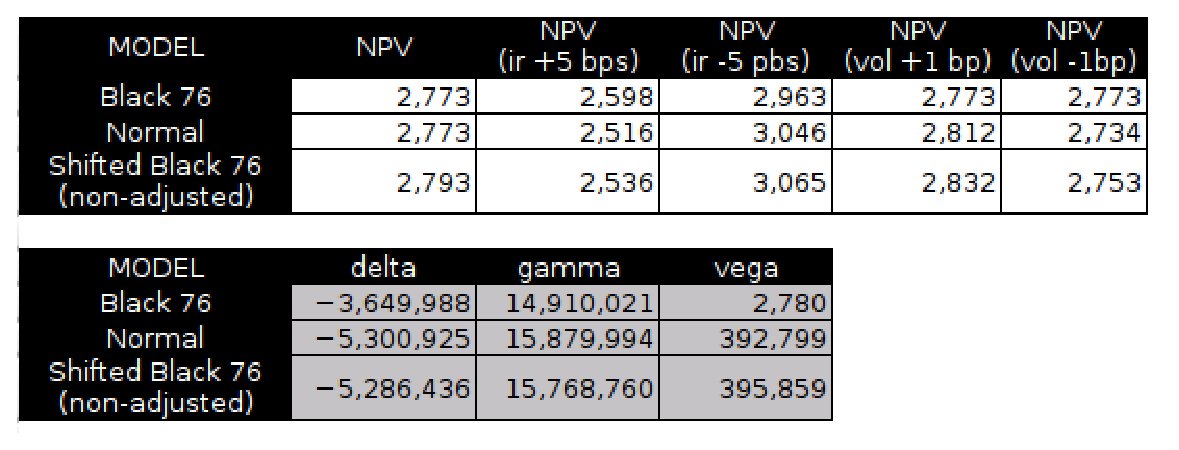
\includegraphics[scale = 0.50]{greeks.eps}
\caption{Caplet Greeks}
\label{greeks}
\end{figure} 
\end{frame}

\begin{frame}{Calculating Greeks}
\setbeamertemplate{itemize items}[ball]
Conclusions of the results from the table are following.
\begin{itemize}
\item Black 76 model shifted by 100\% is a reasonable approximation of normal model.
\item Huge difference in vega between Black 76 and normal model is probably not shocking if one realizes that volatilities under the two models are defined in a completely different way, i.e. in relative vs absolute terms.
\item Gamma, even though not completely the same, is comparable under both models.
\item Difference in deltas might be somewhat surprising - if interest rates increase by +100 bps (assuming everything else constant), caplet value drops by -3.65 MEUR under Black 76 model and by -5.30 MEUR under normal model. In other words, PnL impact depends not only on interest rates but also on a model! As discussed above, this is due to the fact that interest rates are modelled differently and therefore interest rate change of 100 bps has different effect under the two models.
\end{itemize}
\end{frame}

\section{Literature and References}

\begin{frame}{Literature and References}
\setbeamertemplate{itemize items}[ball]
\begin{itemize}
\item [1] Option, Futures, and Other Derivatives - John C. Hull, 5th edition
\item [2] New Volatility Conventions in Negative Interest Environment - d-fine 2012
\item [3] The New Normal - Using the Right Volatility Quote in Times of Low Interest Rates for Solvency II Risk Factor Modelling - Milliman, September 2015
\item [4] Shifted Black-Scholes Model in RiskPro - Michal Mackanic, December 2015
\end{itemize}
\end{frame}

\end{document}
